\documentclass[12pt]{beamer}
\usetheme{CambridgeUS}
\usepackage[utf8]{inputenc}
\usepackage{amsmath}
\usepackage{amsfonts}
\usepackage{amssymb}
\author{Wang,Zhu and Ma}
\title{Optimal Subsampling for Large Sample Logistic Regression}
%\setbeamercovered{transparent} 
%\setbeamertemplate{navigation symbols}{} 
%\logo{} 
%\institute{} 
%\date{} 
%\subject{} 
\begin{document}

\begin{frame}
\titlepage
\end{frame}

%\begin{frame}
%\tableofcontents
%\end{frame}

\begin{frame}{Introduction}
If data is too big, there are several things you can do:
\begin{itemize}
\item Operate on a super computer 
\item Split the data for distributed analysis
\item Downsize the data : Subsampling
\end{itemize}
\end{frame}


\begin{frame}{Review:Logistic Regression}
Given covariates $\mathbf{x}_i\in \mathbb{R}$, logistic regression models are of the form
$$
P\left(y_{i}=1 | \mathbf{x}_{i}\right)=p_{i}(\boldsymbol{\beta})=\frac{\exp \left(\mathbf{x}_{i}^{T} \boldsymbol{\beta}\right)}{1+\exp \left(\mathbf{x}_{i}^{T} \boldsymbol{\beta}\right)}, \quad i=1,2, \ldots, n,
$$
where $y_i \in \{0,1\}$ are the responses and $\mathbf{\beta}$ is a $d\times 1$ vector of unknown parameters. 
\end{frame}

\begin{frame}{Review:Logistic Regression}
The unknown parameter $\mathbf{\beta}$ is often estimated by the
maximum likelihood estimator (MLE) through maximizing the
log-likelihood function with respect to $\mathbf{\beta}$, namely,
$$
\begin{aligned}
\hat{\boldsymbol{\beta}}_{\mathrm{MLE}} &=\arg \max _{\beta} \ell(\boldsymbol{\beta}) \\
&=\arg \max _{\beta} \sum_{i=1}^{n}\left[y_{i} \log p_{i}(\boldsymbol{\beta})+\left(1-y_{i}\right) \log \left\{1-p_{i}(\boldsymbol{\beta})\right\}\right]
\end{aligned}
$$
Analytically, there is no general closed-form solution to the
MLE $\hat{\mathbf{\beta}}_{MLE}$ and iterative procedures are often adopted to find it numerically.
\end{frame}


\begin{frame}{Review:Logistic Regression}
A commonly used iterative procedure is Newton’s
method. Specifically for logistic regression, Newton’s method
iteratively applies the following formula until $\hat{\mathbf{\beta}}^{(t+1)}$ converges
$$
\hat{\beta}^{(t+1)}=\hat{\beta}^{(t)}+\left\{\sum_{i=1}^{n} w_{i}\left(\hat{\beta}^{(t)}\right) \mathbf{x}_{i} \mathbf{x}_{i}^{T}\right\}^{-1} \frac{\partial \ell\left(\hat{\boldsymbol{\beta}}^{(t)}\right)}{\partial \boldsymbol{\beta}},
$$
where $w_{i}(\boldsymbol{\beta})=p_{i}(\boldsymbol{\beta})\left\{1-p_{i}(\boldsymbol{\beta})\right\}$.
\end{frame}

\iffalse
\begin{frame}{Subsampling:OLS}
There are numerous variants of subsampling
algorithms to solve the ordinary least squares (OLS)
in linear regression for large datasets,see
\begin{itemize}
\item Drineas, Mahoney, andMuthukrishnan (2006)
\item Drineas et al. (2011)
\item Ma,Mahoney,and Yu (2014), 
\item Ma, Mahoney, and Yu (2015), 
\item Ma and Sun (2015)
\item  others.
\end{itemize}
\end{frame}
\fi
\section{General Subsampling Algorithm and its Asymptotic Properties}
\begin{frame}{General Subsampling Algorithm}
\begin{itemize}
\item Sampling: Assign subsampling probabilities $\pi_{i},i=1,2,\dots,n$ for all data points. Draw a random subsample
of size $r (\ll n)$ according to the probabilities $\{\pi_i\}_{i=1}^n$ from the full data. Denote the covariates, responses, and
subsampling probabilities in the subsample as $\mathbf{x}_i^{*}, y_i^{*}$ and $\pi_i^{*}$ for $i=1,2,\dots,r$. 
\item Estimation: Maximize
$$
\ell^{*}(\boldsymbol{\beta})=\frac{1}{r} \sum_{i=1}^{r} \frac{1}{\pi_{i}^{*}}\left[y_{i}^{*} \log p_{i}^{*}(\boldsymbol{\beta})+\left(1-y_{i}^{*}\right) \log \left\{1-p_{i}^{*}(\boldsymbol{\beta})\right\}\right]
$$
where $p_i^{*}(\mathbf{\beta})=\exp \left(\boldsymbol{\beta}^{T} \mathbf{x}_{i}^{*}\right) /\left\{1+\exp \left(\boldsymbol{\beta}^{T} \mathbf{x}_{i}^{*}\right)\right\}$.
\end{itemize}
\end{frame}

\begin{frame}{Continue: General Subsampling Algorithm}
Due to the convexity of $\ell^{*}(\mathbf{\beta})$, themaximization can be implemented by Newton’s method, that is, iteratively applying the following formula until convergence
$$
\tilde{\boldsymbol{\beta}}^{(t+1)}=\tilde{\boldsymbol{\beta}}^{(t)}+\left\{\sum_{i=1}^{r} \frac{w_{i}^{*}\left(\tilde{\boldsymbol{\beta}}^{(t)}\right) \mathbf{x}_{i}^{*}\left(\mathbf{x}_{i}^{*}\right)^{T}}{\pi_{i}^{*}}\right\}^{-1} \sum_{i=1}^{r} \frac{\left\{y_{i}^{*}-p_{i}^{*}\left(\tilde{\boldsymbol{\beta}}^{(t)}\right)\right\} \mathbf{x}_{i}^{*}}{\pi_{i}^{*}}
$$
where $w_{i}^{*}(\boldsymbol{\beta})=p_{i}^{*}(\boldsymbol{\beta})\left\{1-p_{i}^{*}(\boldsymbol{\beta})\right\}$.
\end{frame}

\begin{frame}{Assumptions}
Denote the full data matrix as 
$$\mathcal{F}_{n}=(\mathbf{X}, \mathbf{y}), \text { where } \mathbf{X}=\left(\mathbf{x}_{1}, \mathbf{x}_{2}, \ldots, \mathbf{x}_{n}\right)^{T}
$$

\textbf{Assumption 1:} As $ n\to \infty$, $\mathbf{M}_{X}=n^{-1} \sum_{i=1}^{n} w_{i}\left(\hat{\boldsymbol{\beta}}_{\mathrm{MLE}}\right) \mathbf{x}_{i} \mathbf{x}_{i}^{T}$ goes to a positive-definite matrix in probability and $n^{-1} \sum_{i=1}^{n}\left\|\mathbf{x}_{i}\right\|^{3}=O_{P}(1)$.

\textbf{Assumption 2:} $n^{-2} \sum_{i=1}^{n} \pi_{i}^{-1}\left\|\mathbf{x}_{i}\right\|^{k}=O_{P}(1) \text { for } k=2,4$. 
\end{frame}

\begin{frame}{Theorem 1}
If assumptions 1 and 2 hold, then as $n \to \infty$ and $r\to \infty$, $\tilde{\mathbf{\beta}}$ is consistent to $\hat{\mathbf{\beta}}_{MLE}$ in conditional probability, given $\mathcal{F}_n$ in probability. Moreover, the rate of convergence is $r^{-1/2}$. That is, with probability approaching one, for any $\epsilon>0$, there exists a finite $\Delta_{\epsilon}$ and $r_{\epsilon}$ such that
$$
P\left(\left\|\tilde{\boldsymbol{\beta}}-\hat{\boldsymbol{\beta}}_{\mathrm{MLE}}\right\| \geq r^{-1 / 2} \Delta_{\epsilon} | \mathcal{F}_{n}\right)<\epsilon
$$
for all $r\ge r_{\epsilon}$.
\end{frame}

\begin{frame}{Assumption 3.} There exists some $\delta>0$ such that 
$$
n^{-(2+\delta)} \sum_{i=1}^{n} \pi_{i}^{-1-\delta}\left\|\mathbf{x}_{i}\right\|^{2+\delta}=O_{P}(1).
$$
Assumption 3 is used to verify the Lindeberg-Feller condition.

The aforementioned three assumptions are essentially
moment conditions and are very general.
\end{frame}

\begin{frame}{Theorem 2}
If Assumptions 1,2 and 3 hold, then as $n \to \infty$ and $r\to \infty$, conditional on $\mathcal{F}_n$ in probability, 
$$
\mathbf{V}^{-1 / 2}\left(\tilde{\boldsymbol{\beta}}-\hat{\boldsymbol{\beta}}_{\mathrm{MLE}}\right) \stackrel{d}{\to} N(0, \mathbf{I}),
$$
where
$$
\mathbf{V}=\mathbf{M}_{X}^{-1} \mathbf{V}_{c} \mathbf{M}_{X}^{-1}=O_{p}\left(r^{-1}\right),
$$
and 
$$
\mathbf{V}_{c}=\frac{1}{r n^{2}} \sum_{i=1}^{n} \frac{\left\{y_{i}-p_{i}\left(\hat{\boldsymbol{\beta}}_{\mathrm{MLE}}\right)\right\}^{2} \mathbf{x}_{i} \mathbf{x}_{i}^{T}}{\pi_{i}}.
$$
\end{frame}

\section{Optimal Subsampling Strategies}
\begin{frame}{Optimal Subsampling Strategies}
\begin{itemize}
\item To implement Algorithm 1, one has to specify the subsampling
probability (SSP) $\boldsymbol{\pi}=\left\{\pi_{i}\right\}_{i=1}^{n}$ for the full data.
\item An easy choice
is to use the uniform SSP $\pi^{\mathrm{UNI}}=\left\{\pi_{i}=n^{-1}\right\}_{i=1}^{n}$.
\item However, an
algorithm with the uniform SSP may not be 'optimal' and a
nonuniform SSP may have a better performance.
\item In this section,
we propose more efficient subsampling procedures by choosing
nonuniform $\pi_i$'s to “'minimize' the asymptotic variance-covariance
matrix $\mathbf{V}$.
\end{itemize}
\end{frame}

\begin{frame}{Minimum Asymptotic MSE of $\tilde{\beta}$.}
The distribution of $\tilde{\mathbf{\beta}}-\hat{\mathbf{\beta}}_{MLE}$ given $\mathcal{F}$ can be approximately by that of $\mathbf{u}$, a normal variable with distribution $N(0,\mathbf{V})$.

The asymptotic MSE of $ \tilde{\beta}$ is equal to the trace of $\mathbf{V}$, namely
$$
\operatorname{AMSE}(\tilde{\boldsymbol{\beta}})=\mathrm{E}\left(\|\mathbf{u}\|^{2} | \mathcal{F}_{n}\right)=\operatorname{tr}(\mathbf{V})
$$
\end{frame}

\begin{frame}{Theorem 3}
In algorithm 1, if the SSP is chosen such that
$$
\pi_{i}^{\mathrm{mMSE}}=\frac{\left|y_{i}-p_{i}\left(\hat{\boldsymbol{\beta}}_{\mathrm{MLE}}\right)\right|\left\|\mathbf{M}_{X}^{-1} \mathbf{x}_{i}\right\|}{\sum_{j=1}^{n}\left|y_{j}-p_{j}\left(\hat{\boldsymbol{\beta}}_{\mathrm{MLE}}\right)\right|\left\|\mathbf{M}_{X}^{-1} \mathbf{x}_{j}\right\|}, \quad i=1,2, \ldots, n
$$
then asymptotic MSE of $\tilde{\beta}$, $tr(\mathbf{V})$, attains its minimum.
\end{frame}

\begin{frame}{Remarks about Theorem 3}
\begin{itemize}
\item the optimal SSP depends on data through both the covariates and the responses directly.
\item For the covariates, the optimal SSP is larger for a larger $\left\|\mathbf{M}_{X}^{-1} \mathbf{x}_{i}\right\|$, which is the square root of the ith diagonal element
of the matrix $\mathbf{X} \mathbf{M}_{X}^{-2} \mathbf{X}^{T}$.
\item The effect of the responses on the optimal
SSP depends on discrimination difficulties through the term $\left|y_{i}-p_{i}\left(\hat{\boldsymbol{\beta}}_{\mathrm{MLE}}\right)\right|$.
\end{itemize}
\end{frame}

\begin{frame}{The effect of the responses}
Let $S_0=\{i: y_i=0\}$ and $S_1=\{ i:y_i=1\}$.
\begin{itemize}
\item For the $S_0$ set, a larger $p_{i}(\hat{\boldsymbol{\beta}}_{\mathrm{MLE}})$  results in a larger $\pi_{i}^{\mathrm{mMSE}}$.
\item While for the $S_1$ set, the effect is negative.
\item The optimal
subsampling approach is more likely to select data points with
smaller $p_{i}(\hat{\beta}_{MLE})$ when $y_i=1$ and data points with larger $p_{i}(\hat{\beta}_{MLE})$ when $y_i=0$
\item Intuitively, it attempts to give preferences
to data points that are more likely to be misclassified.
\end{itemize} 
\end{frame}

\begin{frame}{The effect of the responses}
$$
\begin{aligned}
\operatorname{tr}(\mathbf{V}) &=\frac{1}{r n^{2}} \operatorname{tr}\left(\sum_{i=1}^{n} \frac{\left\{y_{i}-p_{i}\left(\hat{\boldsymbol{\beta}}_{\mathrm{MLE}}\right)\right\}^{2} \mathbf{M}_{X}^{-1} \mathbf{x}_{i} \mathbf{x}_{i}^{T} \mathbf{M}_{X}^{-1}}{\pi_{i}}\right) \\
&=\frac{1}{r n^{2}} \sum_{i=1}^{n} \frac{\left\{y_{i}-p_{i}\left(\hat{\boldsymbol{\beta}}_{\mathrm{MLE}}\right)\right\}^{2} \operatorname{tr}\left(\mathbf{M}_{X}^{-1} \mathbf{x}_{i} \mathbf{x}_{i}^{T} \mathbf{M}_{X}^{-1}\right)}{\pi_{i}} \\
&= \frac{1}{r n^{2}} \sum_{i \in S_{0}} \frac{\left\{p_{i}\left(\hat{\boldsymbol{\beta}}_{\mathrm{MLE}}\right)\right\}^{2}\left\|\mathbf{M}_{X}^{-1} \mathbf{x}_{i}\right\|^{2}}{\pi_{i}}\\
&\quad +\frac{1}{r n^{2}} \sum_{i \in S_{1}} \frac{\left\{1-p_{i}\left(\hat{\boldsymbol{\beta}}_{\mathrm{MLE}}\right)\right\}^{2}\left\|\mathbf{M}_{X}^{-1} \mathbf{x}_{i}\right\|^{2}}{\pi_{i}}
\end{aligned}
$$
\end{frame}

\begin{frame}{Minimum Asymptotic MSE of $M_X\tilde{\beta}$}
For two given SSPs $\boldsymbol{\pi}^{(1)}$ and $\boldsymbol{\pi}^{(2)}$, $\mathbf{V}\left(\boldsymbol{\pi}^{(1)}\right) \leq \mathbf{V}\left(\boldsymbol{\pi}^{(2)}\right)$ if and only if 
$\mathbf{V}_c\left(\boldsymbol{\pi}^{(1)}\right) \leq \mathbf{V}_c\left(\boldsymbol{\pi}^{(2)}\right)$

This gives us guidance to simplify the optimality criterion.

Instead of focusing on the more complicated
matrix $\mathbf{V}$, we define an alternative optimality criterion by
focusing on $\mathbf{V}_c$. 

Specifically, instead of minimizing $tr(\mathbf{V})$, we choose to minimize $tr(\mathbf{V}_c)$.
\end{frame}

\begin{frame}{Theorem 4}
In Algorithm 1, if the SSP is chosen such that
$$
\pi_{i}^{\mathrm{mVc}}=\frac{\left|y_{i}-p_{i}\left(\hat{\boldsymbol{\beta}}_{\mathrm{MLE}}\right)\right|\left\|\mathbf{x}_{i}\right\|}{\sum_{j=1}^{n}\left|y_{j}-p_{j}\left(\hat{\boldsymbol{\beta}}_{\mathrm{MLE}}\right)\right|\left\|\mathbf{x}_{j}\right\|}, \quad i=1,2, \ldots, n
$$
then $tr(\mathbf{V}_c)$ attains its minimum.
\end{frame}

\begin{frame}{Remark of Theorem 4}
\begin{itemize}
\item It turns out that the alternative optimality criterion indeed greatly reduces the computing time.
\item $\operatorname{tr}\left(\mathbf{V}_{c}\right)=\mathrm{E}\left(\left\|\mathbf{M}_{X} \mathbf{u}\right\|^{2} | \mathcal{F}_{n}\right)$ is the AMSE of $\mathbf{M}_{X}\tilde{\mathbf{\beta}}$
\end{itemize}
\end{frame}


\begin{frame}{Two step algorithm}
\begin{itemize}
\item The optimal SSP defined before depend on $\hat{\mathbf{\beta}}_{MLE}$,which is the full data MLE to be approximated, so an exact OSMAC is not applicable directly.
\item We propose a two-step algorithm to approximate the
OSMAC.
\item In the first step, a subsample of $r_0$ is taken to get a pilot
estimate of $\hat{\mathbf{\beta}}_{MLE}$ which is then used to approximate the optimal
SSPs for drawing the more informative second step subsample.
\end{itemize}
\end{frame}

\begin{frame}{Two step algorithm}
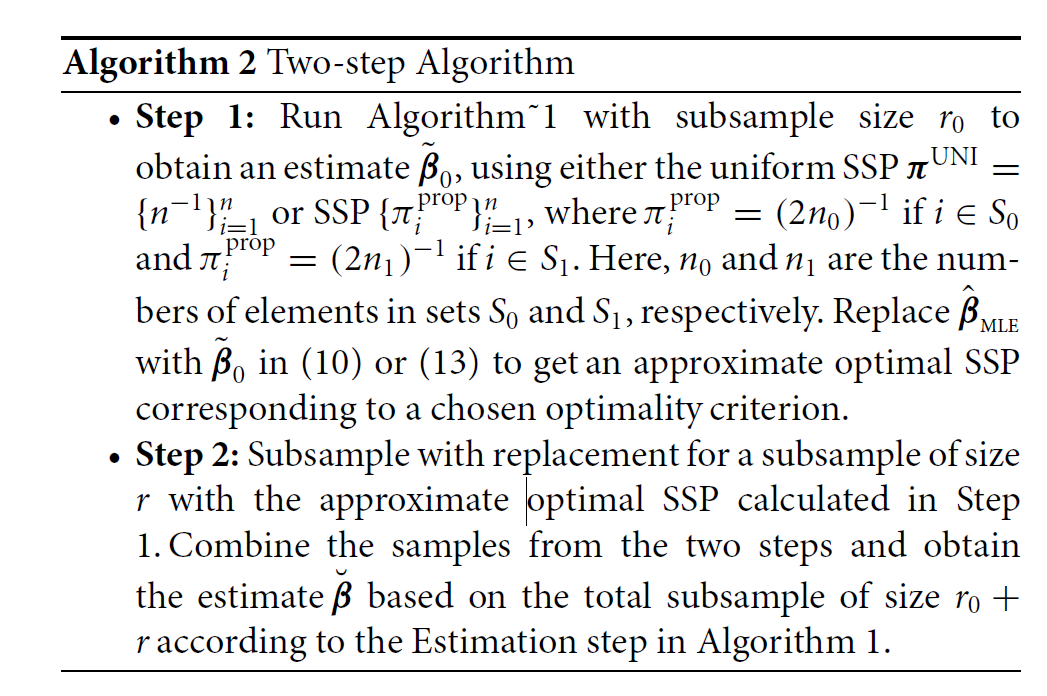
\includegraphics[scale=1]{fig1.png} 
\end{frame}

\begin{frame}{Assumption 4}
The covariate distribution satisfies that $\mathrm{E}\left(\mathbf{x} \mathbf{x}^{T}\right)$ positive definite and $\mathrm{E}\left(e^{\mathrm{a}^{T} \mathrm{x}}\right)<\infty$ for any $\mathbf{a}\in \mathbb{R}^d$.

Assumption 4 imposes two conditions on covariate distribution.
The first condition ensures that the asymptotic covariance
matrix is full rank.
The second condition requires that covariate distributions
have light tails.
\end{frame}

\begin{frame}{Theorem 5}
Let $r_0r^{-1/2} \to 0.$ 0. Under Assumption 4, if the estimate $\tilde{\beta}_0$  based on the first step sample exists, then, as $r\to \infty$ and $n \to \infty$, with probability approaching one, for any $\epsilon>0$, there exists a finite $\delta_{\epsilon}$ and $r_{\epsilon}$ such that
$$
P\left(\left\|\check{\boldsymbol{\beta}}-\hat{\boldsymbol{\beta}}_{\mathrm{MLE}}\right\| \geq r^{-1 / 2} \Delta_{\epsilon} | \mathcal{F}_{n}\right)<\epsilon
$$ 
for all $ r\ge r_{\epsilon}$.
\end{frame}

\begin{frame}{Theorem 6}
Assume that $r_0r^{-1/2} \to 0.$ 0. Under Assumption 4, as $r_0\to \infty, r\to \infty$ and $n \to \infty$,  conditional on $\mathcal{F}_n$ and $\tilde{\beta}_0$,
$$
\mathbf{V}^{-1 / 2}\left(\check{\boldsymbol{\beta}}-\hat{\boldsymbol{\beta}}_{\mathrm{MLE}}\right) \longrightarrow N(0, \mathbf{I})
$$
in distribution, in which $\mathbf{V}=\mathbf{M}_{X}^{-1} \mathbf{V}_{c} \mathbf{M}_{X}^{-1}$ with $\mathbf{V}_c$  having the
expression of
$$
\mathbf{V}_{c}=\frac{1}{r n^{2}}\left\{\sum_{i=1}^{n}\left|y_{i}-p_{i}\left(\hat{\boldsymbol{\beta}}_{\mathrm{MLE}}\right)\right|\left\|\mathbf{x}_{i}\right\|\right\}\left\{\sum_{i=1}^{n} \frac{\left|y_{i}-p_{i}\left(\hat{\boldsymbol{\beta}}_{\mathrm{MLE}}\right)\right| \mathbf{x}_{i} \mathbf{x}_{i}^{T}}{\left\|\mathbf{x}_{i}\right\|}\right\}.
$$
\end{frame}

\section{Simulation}
\begin{frame}{Simulation}
$n=10000$, true $\beta_0$ being a $7 \times 1$ vector of 0.5.
We consider the following six simulated datasets using different distributions of $\mathbf{x}$
\begin{itemize}
\item mznormal. $\mathbf{x}$ follows a multivariate normal distribution $N(\mathbf{0}, \mathbf{\Sigma}), \text { where } \boldsymbol{\Sigma}_{i j}=0.5^{I(i \neq j)}$.
\item nzNormal.  $\mathbf{x}$ follows a multivariate normal distribution $N(1.5,\Sigma)$. About 95\% of the
responses are 1’s, so this dataset is an example of imbalanced
data.
\item ueNormal. $\mathbf{x}$ follows a multivariate normal distribution with zero mean but its components have unequal variances.
\item mixNormal. $\mathbf{x} \sim 0.5 N(\mathbf{1}, \mathbf{\Sigma})+0.5 N(-\mathbf{1}, \mathbf{\Sigma})$.
\item $T_3$ with covariance $\Sigma$
\item EXP independent.

\end{itemize}
\end{frame}


\begin{frame}{Boxplots of SSPs for different datasets}
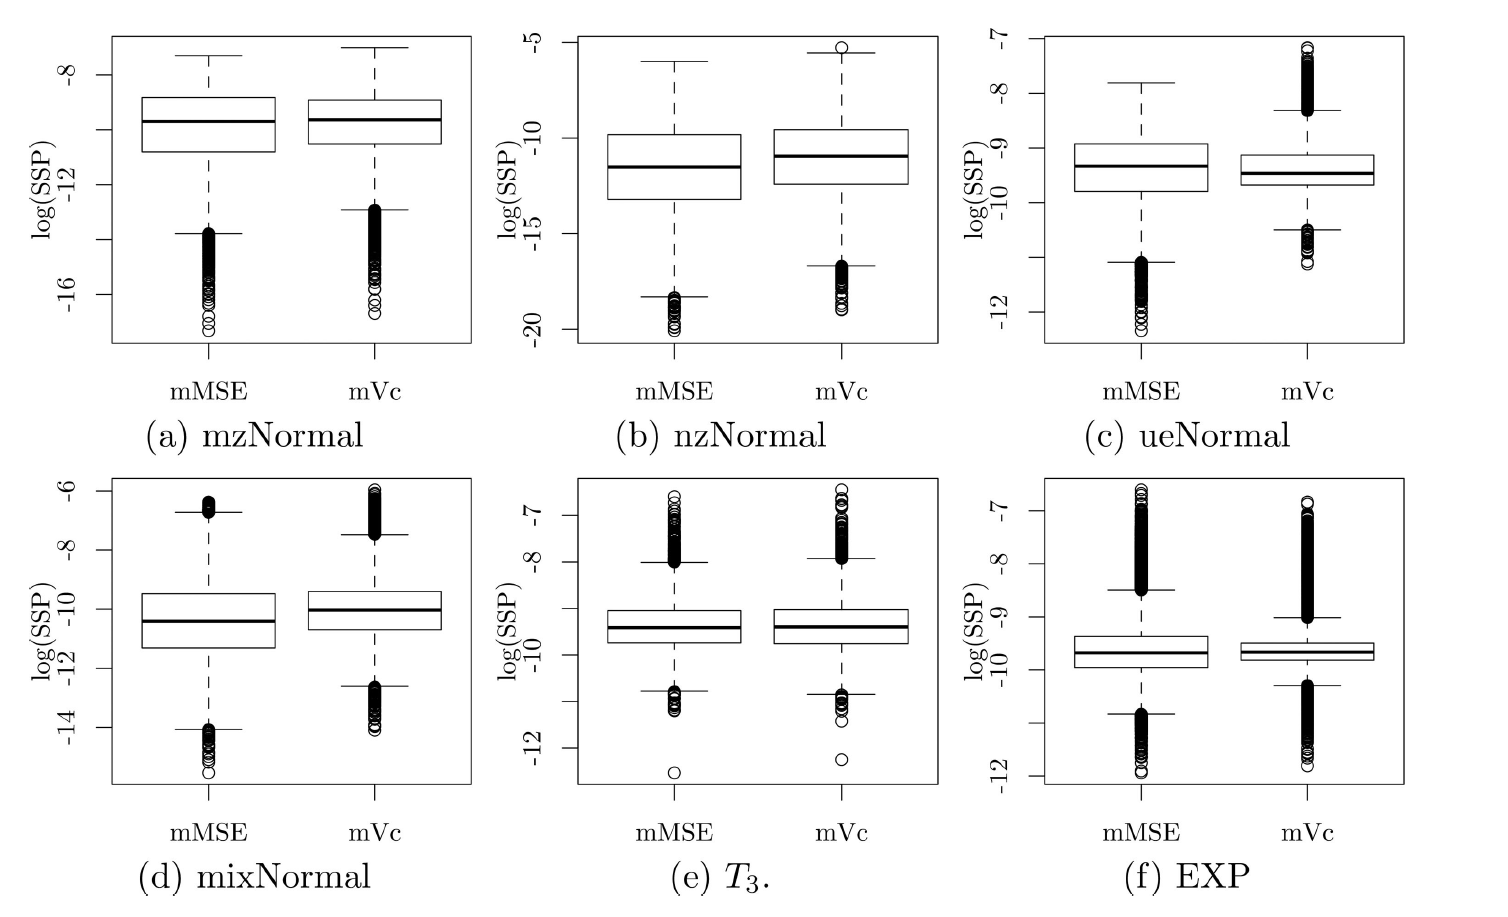
\includegraphics[scale=0.8]{fig2.png} 
\end{frame}

\begin{frame}{MSEs for different second step subsample size r with the first step subsample size being fixed at $r_0=200$.}
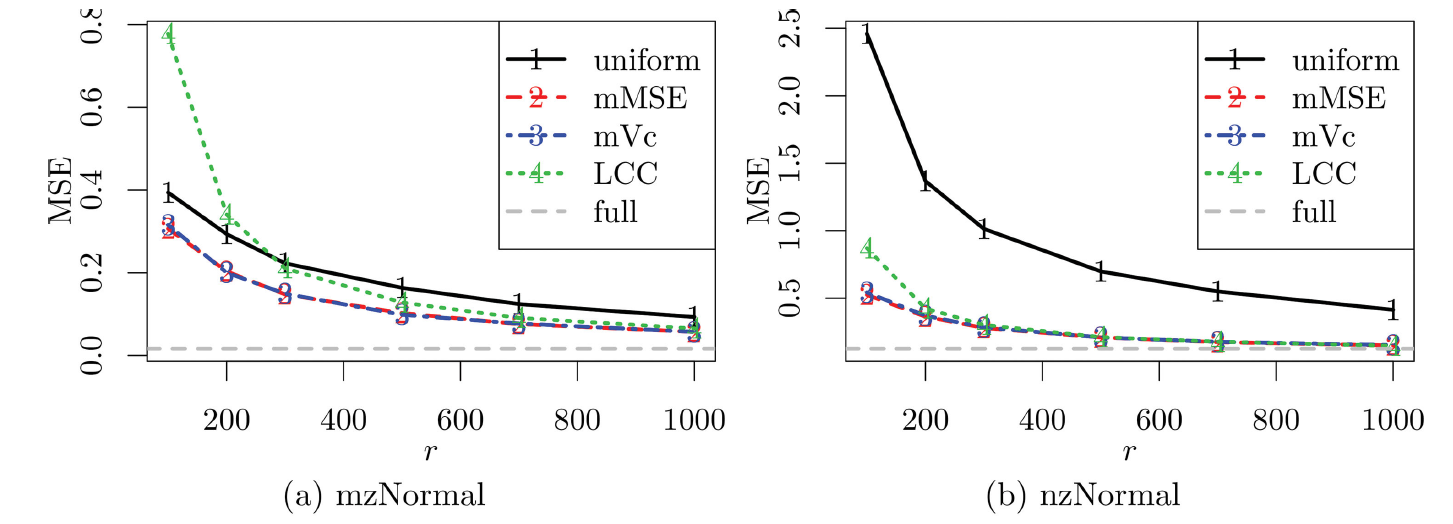
\includegraphics[scale=0.8]{fig3.png} 
\end{frame}

\begin{frame}{Continue}
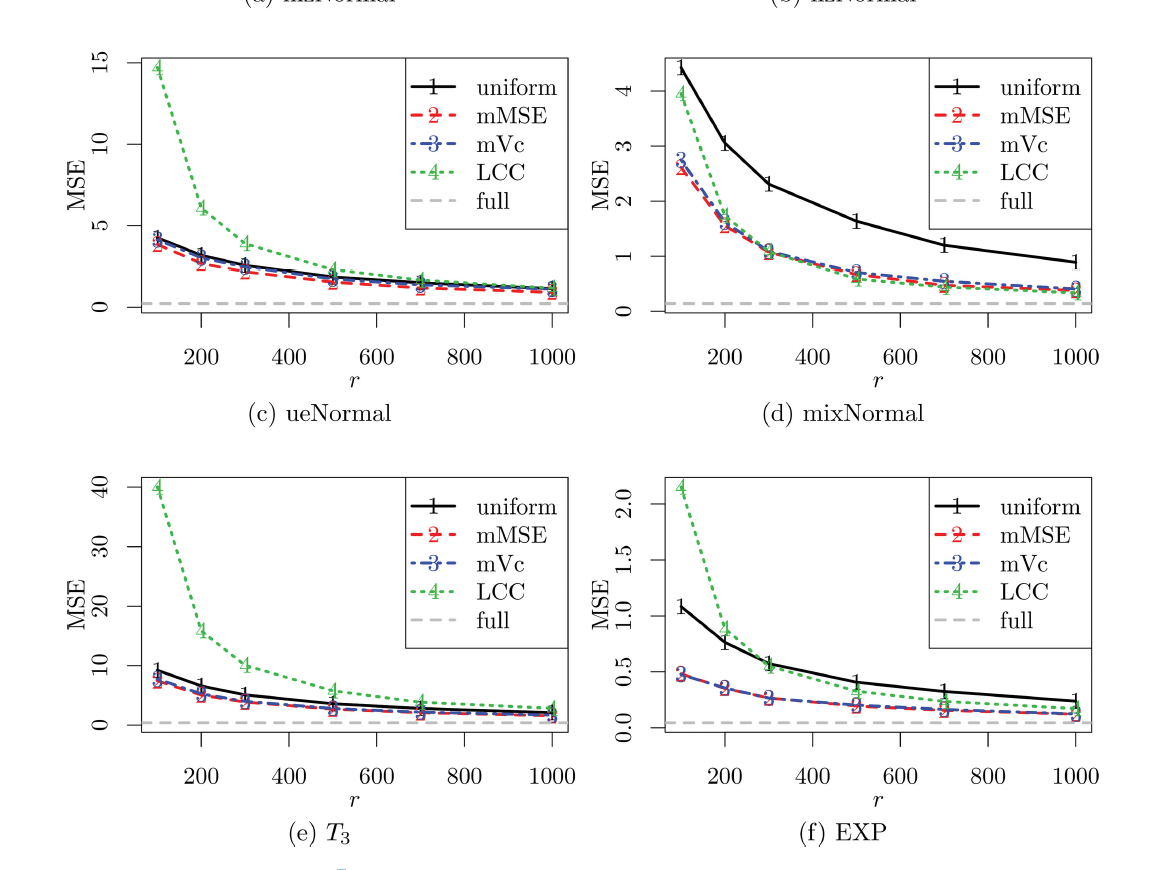
\includegraphics[scale=0.8]{fig4.png} 
\end{frame}

\begin{frame}{Figure 3 MSEs versus proportions of the first step subsample with fixed total subsample sizes for the mzNormal dataset.}
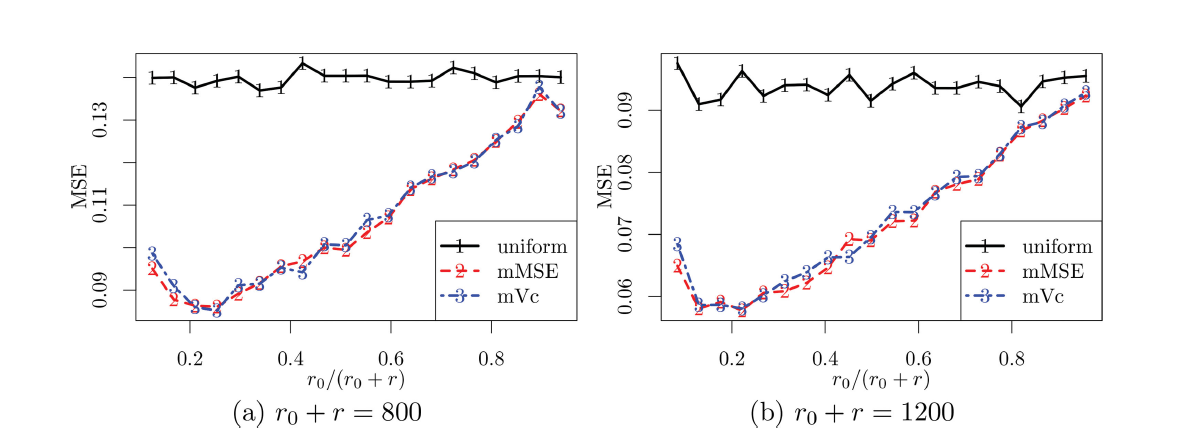
\includegraphics[scale=1]{fig5.png} 
\end{frame}

\begin{frame}{Proportions of correct classifications for different second step subsample size r with the first step subsample size being fixed at $r_0=200$.}
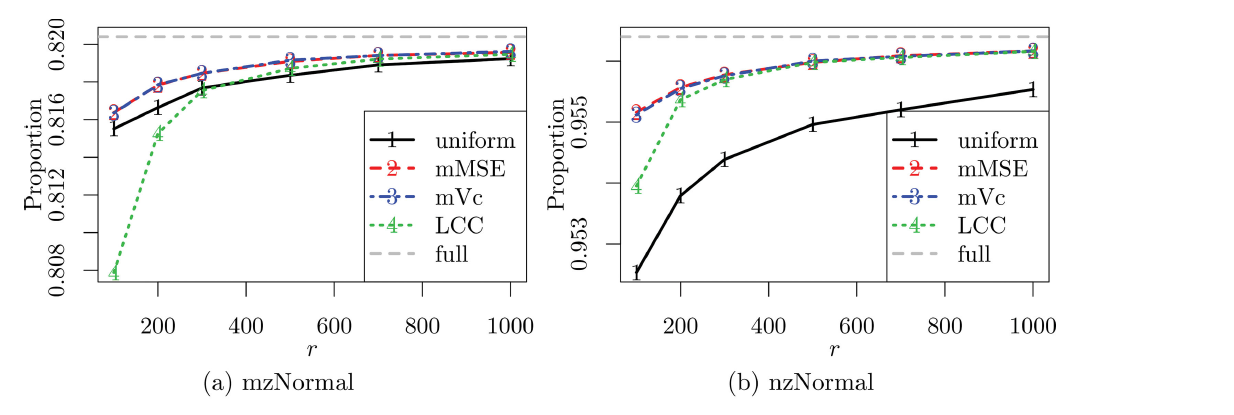
\includegraphics[scale=1]{fig6.png} 
\end{frame}

\begin{frame}{Continue}
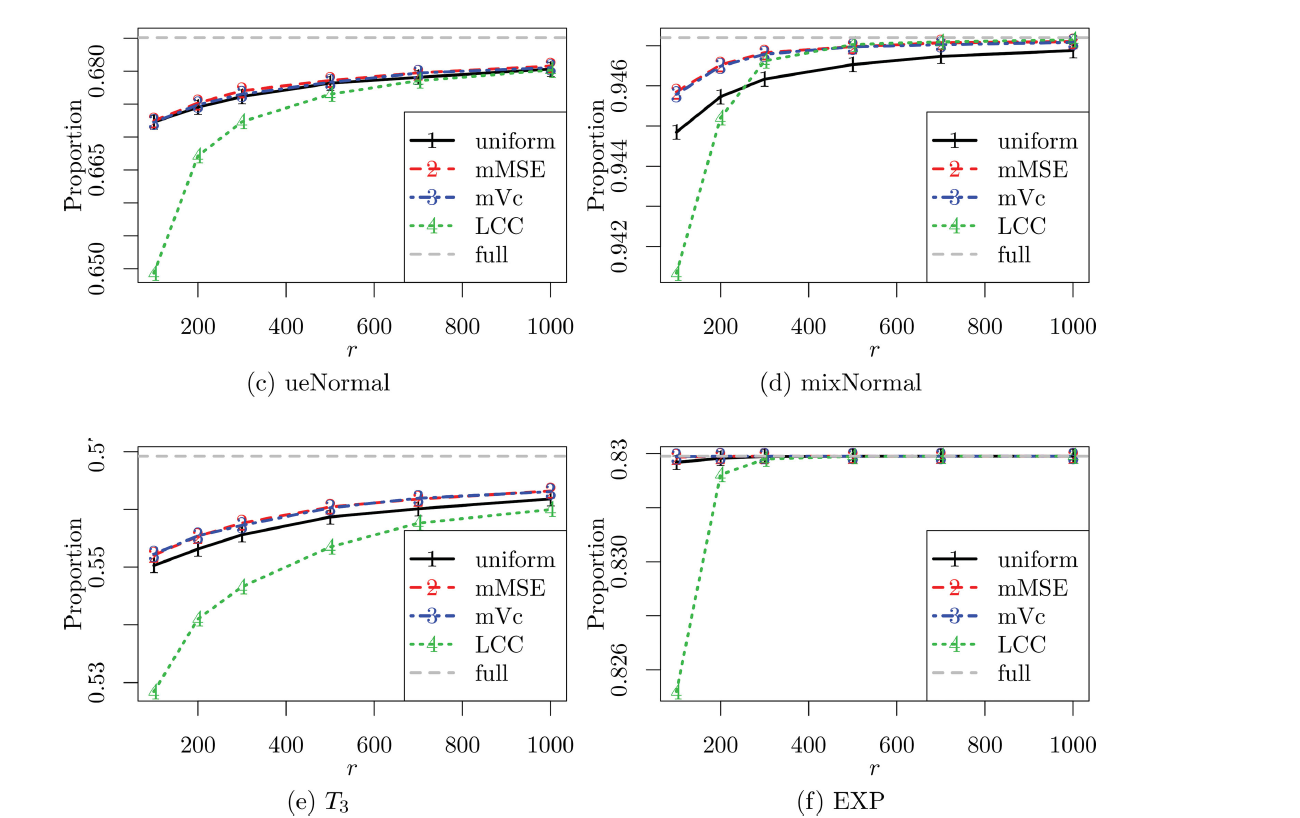
\includegraphics[scale=0.8]{fig7.png} 
\end{frame}

\begin{frame}{Estimated and empirical MSEs for the OSMAC with $\pi^{mMSE}$, The first step subsample size is fixed at $r_0=200$.}
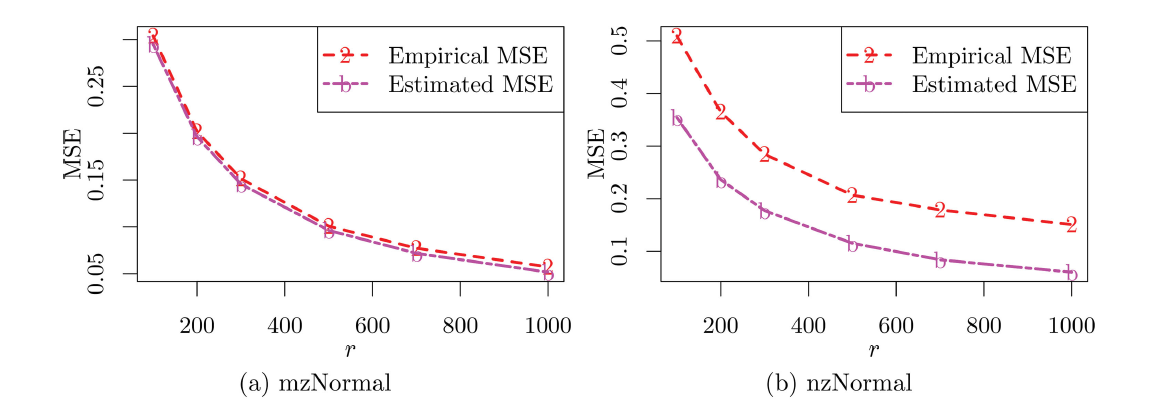
\includegraphics[scale=0.8]{fig8.png} 
\end{frame}

\begin{frame}{Continue}
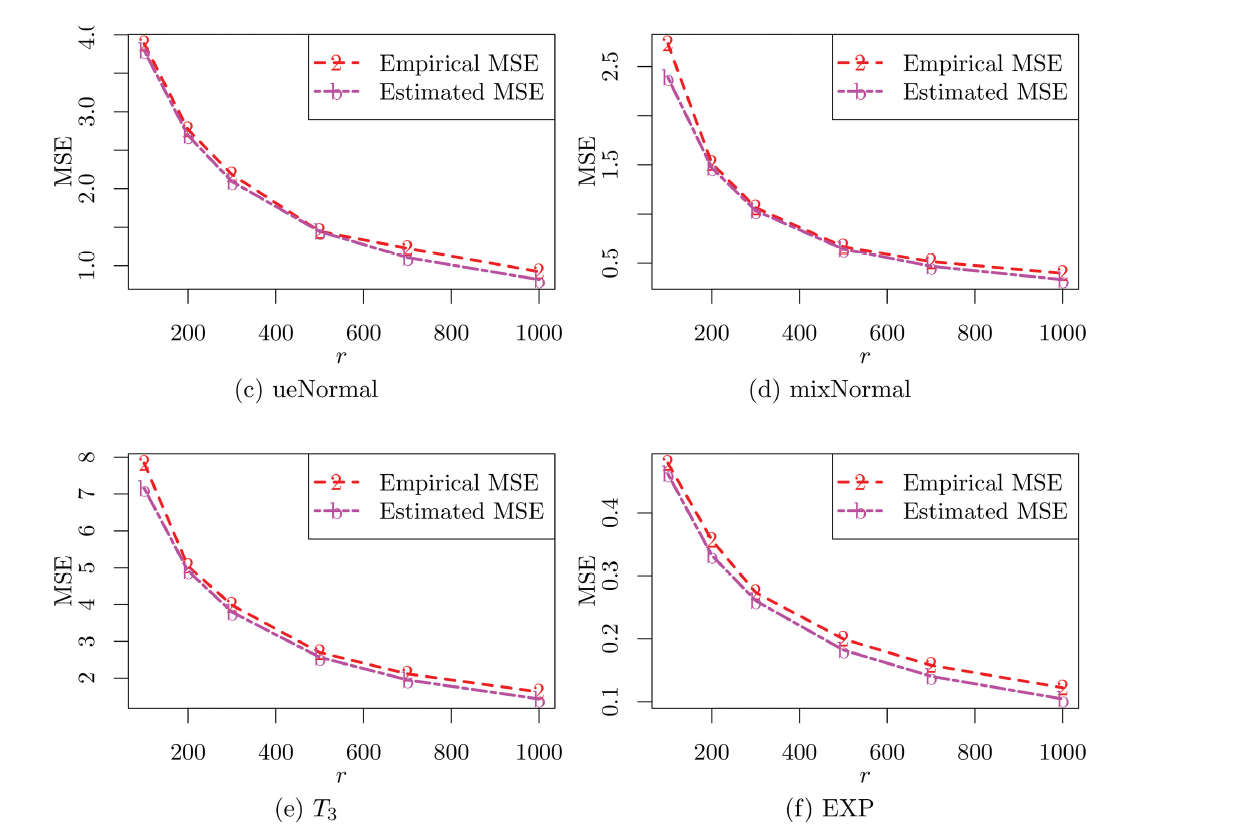
\includegraphics[scale=0.8]{fig9.png} 
\end{frame}


\begin{frame}{Empirical coverage probabilities for different second step subsample size r with the first step subsample size being fixed}
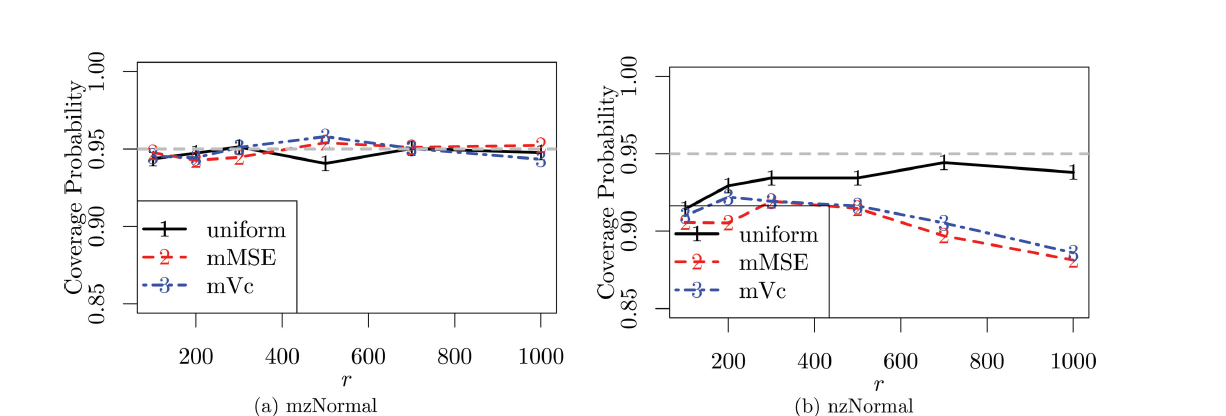
\includegraphics[scale=0.8]{fig10.png} 
\end{frame}

\begin{frame}{Continue}
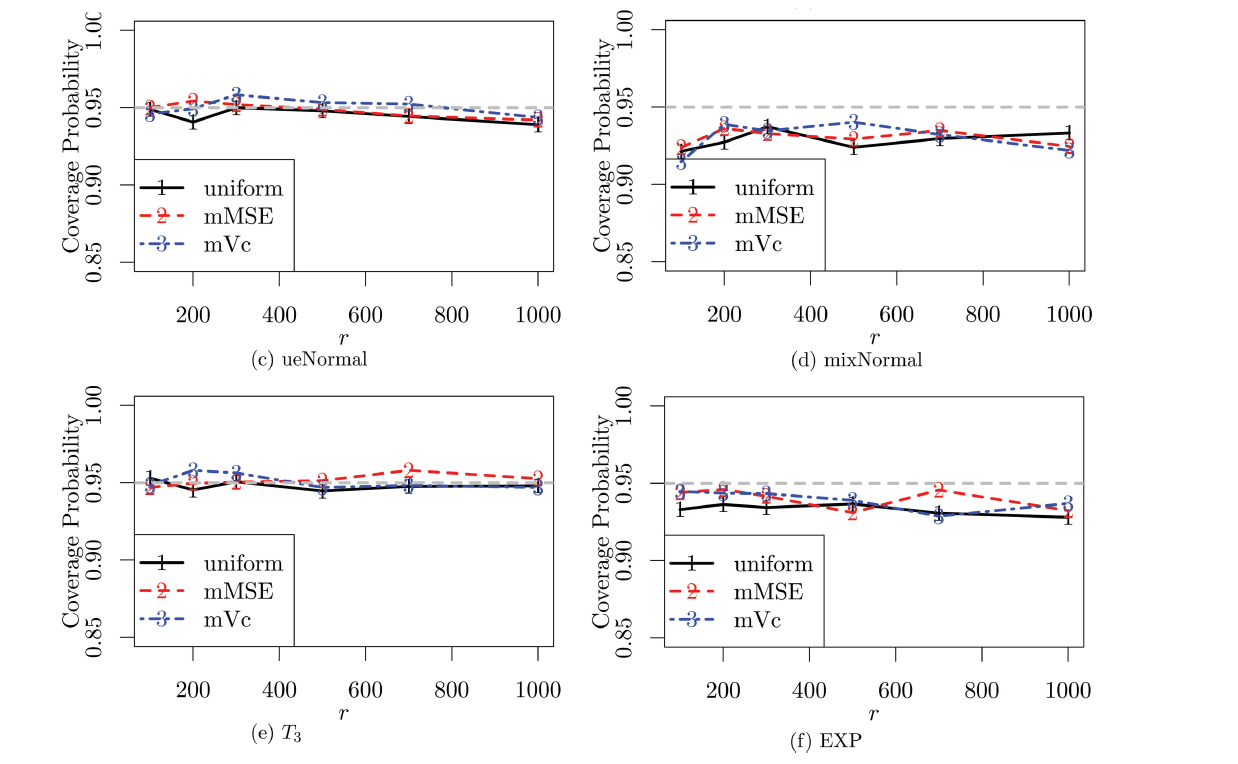
\includegraphics[scale=0.8]{fig11.png} 
\end{frame}


\begin{frame}{Time}
\begin{center}
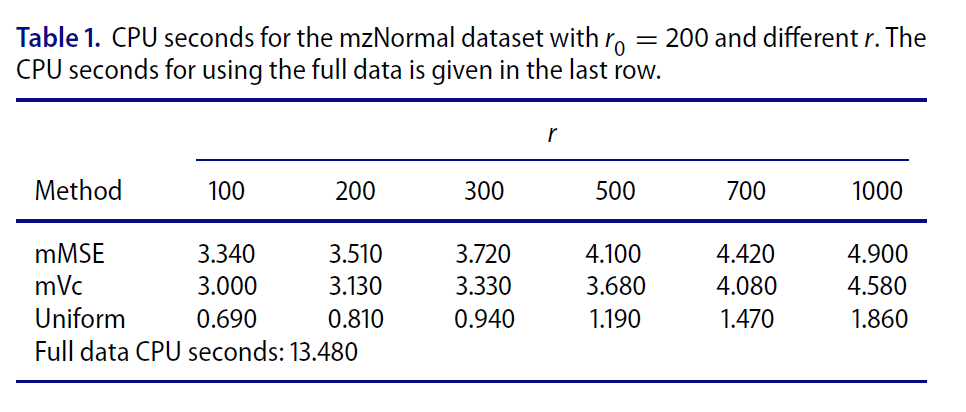
\includegraphics[scale=0.8]{fig12.png} 
\end{center}
\end{frame}


\begin{frame}{Numerical Evaluations for Rare Events data}
To investigate the performance of the proposed method for the
case of rare events, we generate rare events data using the same
configurations that are used to generate the nzNormal data, except we change the mean of $\mathbf{x}$ to -2.14 or -2.9. With
these values, 1.01\% and 0.14\% responses are 1 in the full data of size $n=10000$.
\end{frame}


\begin{frame}
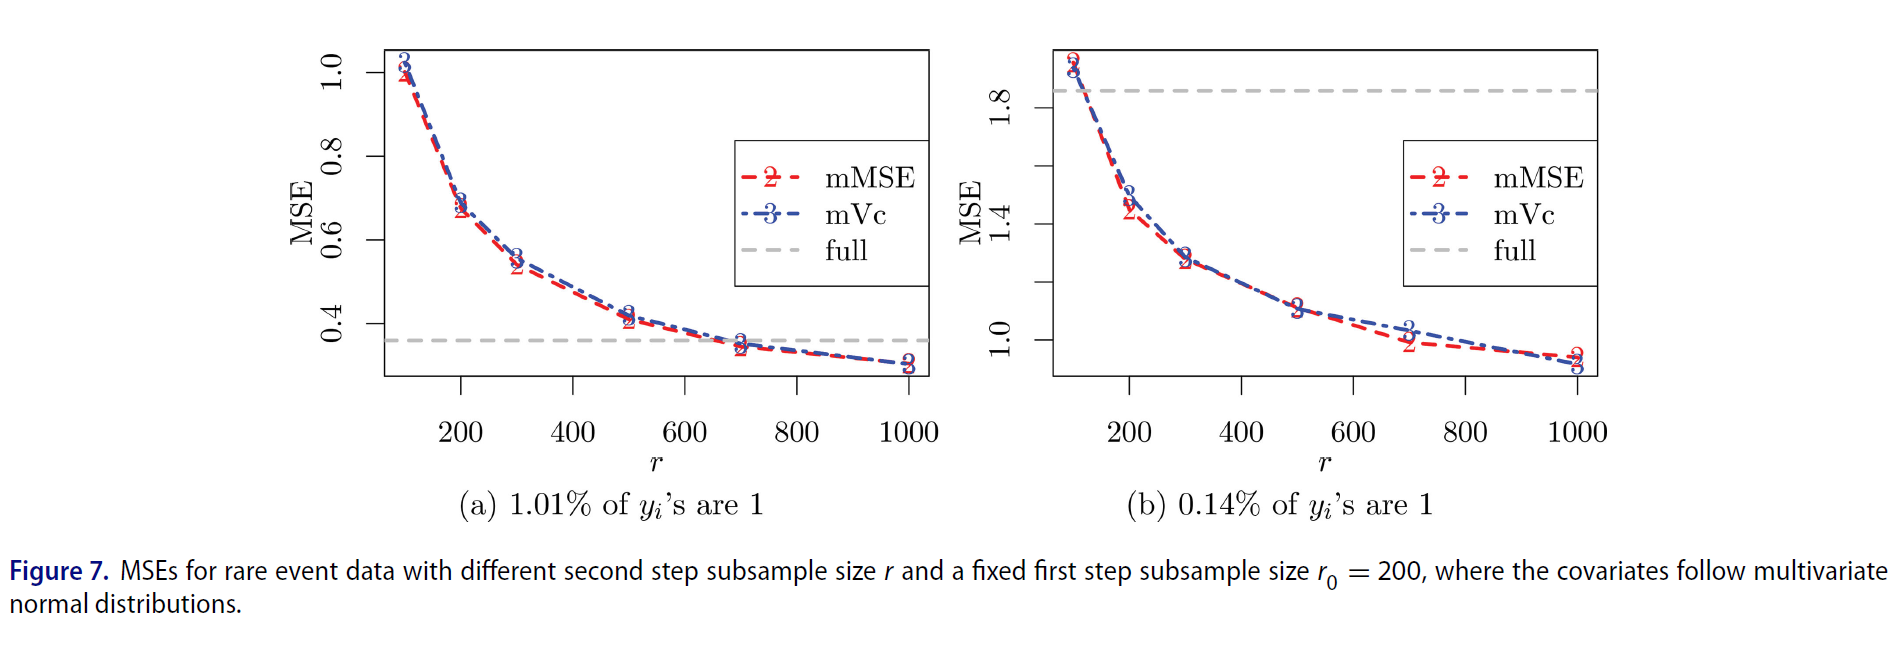
\includegraphics[scale=0.65]{fig13.png} 
\end{frame}

\begin{frame}
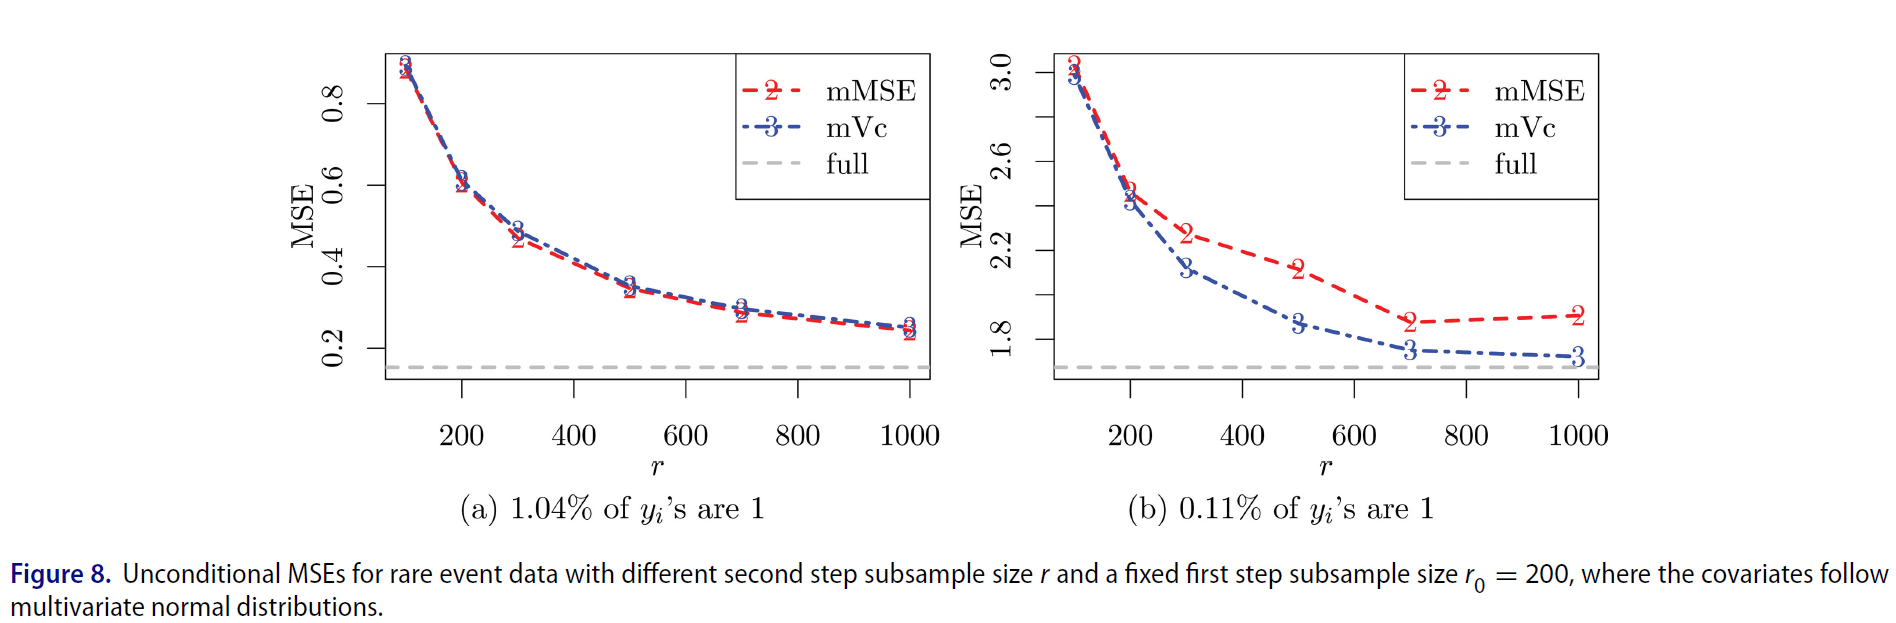
\includegraphics[scale=0.65]{fig14.png} 
\end{frame}

\section{Census Income Dataset}
\begin{frame}{Census Income Dataset}
\begin{itemize}
\item There are totally 48842 observations in the dataset, and the response variable is whether a person's income exceeds \$ 59K a year.
\item There are 11,687 individuals
(23.93\%) in the data whose income exceed \$50K a year.
\item Inferential task is to estimate the effect on income from the following covariates: $x_1$, age; $x_2$, final weight (Fnlwgt); $x_3$, highest
level of education in numerical form; $x_4$, capital loss (LosCap);
$x_5$, hours worked per week. 
\end{itemize}
\end{frame}
\begin{frame}{MSEs and proportions of correct classifications for the adult income dataset with $r_0=200$ and different second step subsample size r}
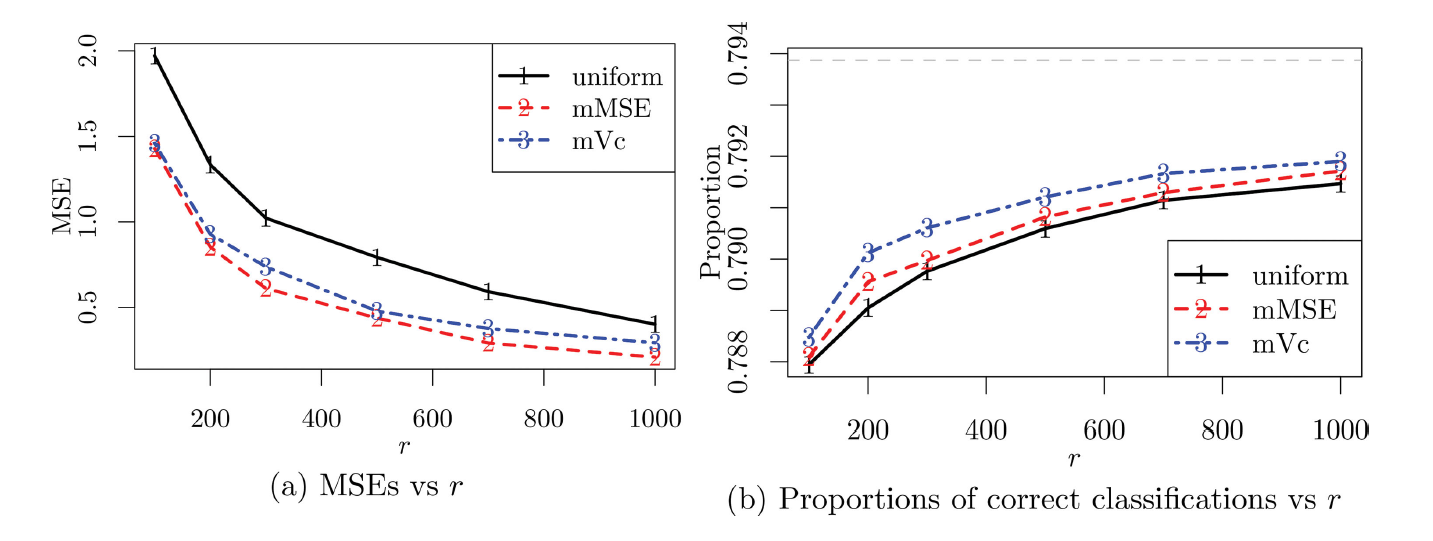
\includegraphics[scale=0.8]{fig15.png} 
\end{frame}

\begin{frame}{Supersymmetric Benchmark Dataset}
\begin{itemize}
\item The full sample size is 5,000,000 and the
data file is about 2.4 gigabytes. 
\item About 54.24\% of the responses in
the full data are fromthe background process. 
\item  We use the first
n = 4,500,000 observation as the training set and use the last
500,000 observations as the validation set.
\end{itemize}
\end{frame}

\begin{frame}{MSEs and proportions of correct classifications for the SUSY dataset with $r_0=200$ and different second step subsample size r.}
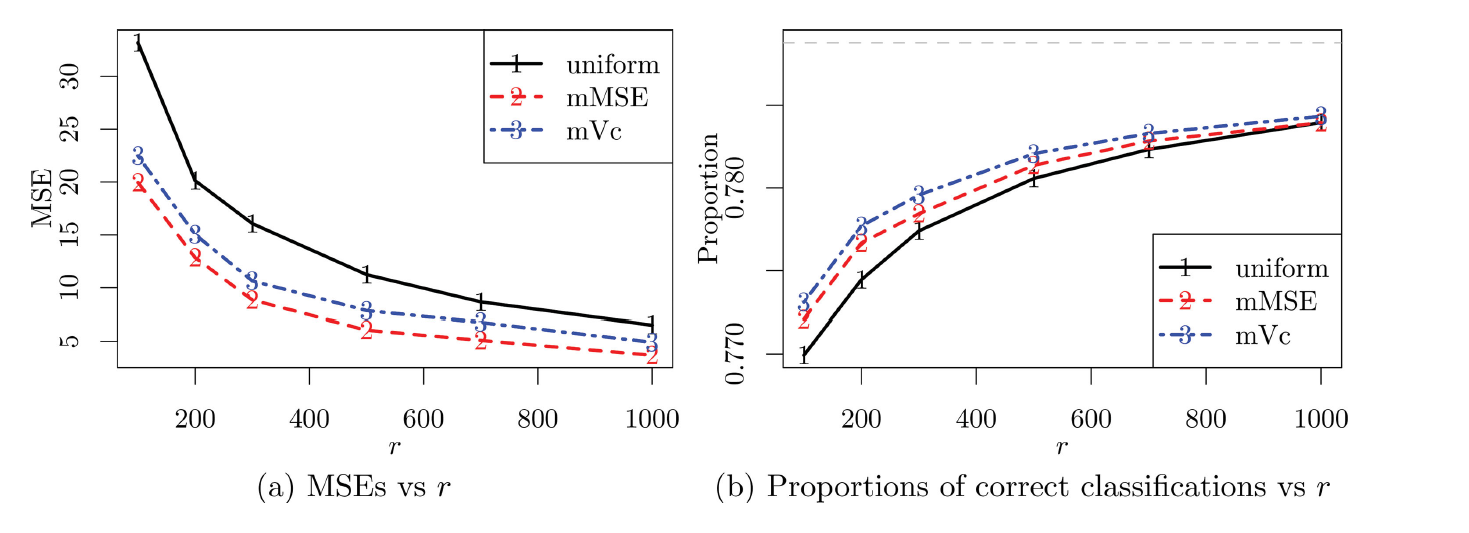
\includegraphics[scale=0.8]{fig16.png} 
\end{frame}

\begin{frame}{Average AUC (as percentage) for the SUSY dataset based on 1000 subsamples.}
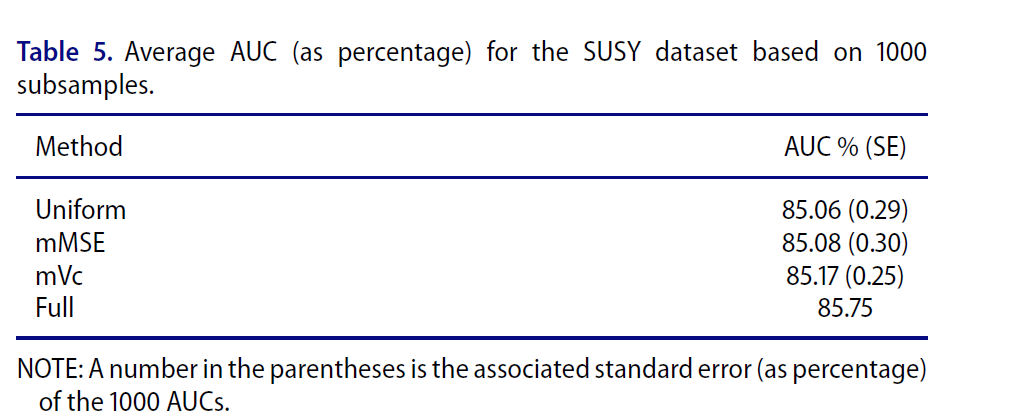
\includegraphics[scale=1]{fig17.png} 
\end{frame}
\end{document}